% =========================================================================
% Self-Supervised Reconstruction-Guided Edge Pruning for Label-Efficient
% Graph Neural Network-based IoT Intrusion Detection
%
% Master's Thesis (research-standard manuscript)
%
% Compile on Overleaf (pdfLaTeX + BibTeX):
%   pdflatex THESIS && bibtex THESIS && pdflatex THESIS && pdflatex THESIS
% =========================================================================
\documentclass[11pt,a4paper]{report}

% --- Layout (tuned to fit a comprehensive Master's thesis in ~30 pages) ---
\usepackage[margin=2.2cm,top=2.2cm,bottom=2.4cm]{geometry}
\usepackage{setspace}
\linespread{1.18}   % between single and 1.5; readable and compact

% --- Encoding & fonts ---
\usepackage[T1]{fontenc}
\usepackage[utf8]{inputenc}
\usepackage{lmodern}
\usepackage{microtype}

% --- Math ---
\usepackage{amsmath, amssymb, amsthm}
\usepackage{bm}
\usepackage{mathtools}

% --- Algorithms ---
\usepackage{algorithm}
\usepackage{algpseudocode}

% --- Graphics, colour, diagrams ---
\usepackage{graphicx}
\usepackage{xcolor}
\usepackage{tikz}
\usetikzlibrary{shapes.geometric, arrows.meta, positioning, fit, backgrounds, calc}

% --- Tables ---
\usepackage{booktabs}
\usepackage{multirow}
\usepackage{array}
\usepackage{tabularx}
\usepackage{makecell}

% --- Captions ---
\usepackage[font=small,labelfont=bf]{caption}
\usepackage[font=footnotesize,labelfont=bf]{subcaption}

% --- Acronyms ---
\usepackage[acronym,nonumberlist,nopostdot]{glossaries}
\makeglossaries

% --- Code listings ---
\usepackage{listings}
\lstdefinestyle{pystyle}{
  language=Python,
  basicstyle=\ttfamily\footnotesize,
  keywordstyle=\color{blue!70!black}\bfseries,
  commentstyle=\color{green!50!black}\itshape,
  stringstyle=\color{red!70!black},
  showstringspaces=false,
  breaklines=true,
  frame=single,
  framesep=4pt,
  backgroundcolor=\color{gray!5},
  numbers=left, numberstyle=\tiny\color{gray}, numbersep=5pt,
}
\lstset{style=pystyle}

% --- Theorem environments ---
\theoremstyle{definition}
\newtheorem{definition}{Definition}[chapter]
\newtheorem{problem}{Problem}[chapter]
\theoremstyle{remark}
\newtheorem{remark}{Remark}[chapter]

% --- Hyperref (load last) ---
\usepackage{hyperref}
\hypersetup{
  colorlinks=true,
  linkcolor=blue!50!black,
  citecolor=teal!60!black,
  urlcolor=blue!60!black,
}

% --- Misc ---
\usepackage{enumitem}
\setlist{topsep=2pt,itemsep=2pt,parsep=0pt}
\usepackage{titlesec}
% Tighter chapter heading: compact "Chapter N" + title on same area
\titleformat{\chapter}[hang]{\Large\bfseries}{\thechapter.\hspace{0.6em}}{0pt}{\Large}
\titlespacing*{\chapter}{0pt}{-10pt}{16pt}
\titlespacing*{\section}{0pt}{12pt}{4pt}
\titlespacing*{\subsection}{0pt}{8pt}{3pt}

% --- TikZ styles ---
\tikzset{
  block/.style={rectangle, rounded corners, draw=black!70,
                fill=blue!7, minimum width=4.5cm, minimum height=1.0cm,
                align=center, font=\small},
  loss/.style={rectangle, draw=black!50, fill=orange!12,
               minimum width=3.0cm, minimum height=0.7cm,
               align=center, font=\footnotesize\itshape},
  data/.style={rectangle, draw=black!50, fill=green!10,
               minimum width=3.0cm, minimum height=0.6cm,
               align=center, font=\footnotesize},
  arrow/.style={-Stealth, thick},
  thinarr/.style={-Stealth, thin, dashed, gray!70},
}

% --- Acronyms ---
\newacronym{gnn}{GNN}{Graph Neural Network}
\newacronym{gcn}{GCN}{Graph Convolutional Network}
\newacronym{ids}{IDS}{Intrusion Detection System}
\newacronym{iot}{IoT}{Internet of Things}
\newacronym{ae}{AE}{Autoencoder}
\newacronym{mse}{MSE}{Mean Squared Error}
\newacronym{ce}{CE}{Cross-Entropy}
\newacronym{ood}{OOD}{Out-of-Distribution}
\newacronym{ste}{ST}{Straight-Through (estimator)}
\newacronym{auc}{AUC-ROC}{Area Under the Receiver Operating Characteristic curve}
\newacronym{f1}{F1}{F1-score (harmonic mean of precision and recall)}

% =========================================================================
\begin{document}

% --- Title Page -----------------------------------------------------------
\begin{titlepage}
\centering
\vspace*{1.5cm}

{\Large\bfseries Self-Supervised Reconstruction-Guided\\[0.3em]
Edge Pruning for Label-Efficient\\[0.3em]
Graph Neural Network-based\\[0.3em]
IoT Intrusion Detection\par}

\vspace{2.0cm}
\rule{0.7\textwidth}{0.5pt}\\[1ex]
{\large \textit{Master's Thesis}}\\[1ex]
\rule{0.7\textwidth}{0.5pt}

\vspace{1.5cm}
{\large Pulkit Mittal \par}

\vspace{2cm}

\begin{tabular}{rl}
\textbf{Domain:}            & Graph Neural Networks $\,\cdot\,$ IoT Security \\
\textbf{Reference baseline:}& Villegas-Ch et al., \emph{IEEE Access} \\
\textbf{Contribution type:} & Methodological (training-supervision design) \\
\textbf{Code artefacts:}    & \texttt{reconstruction\_pruning\_model.py}, \\
                            & \texttt{main\_pipeline.py},
                              \texttt{label\_efficiency\_study.py} \\
\textbf{Data artefacts:}    & Synthetic IoT graph (controllable noise) \\
\end{tabular}

\vfill
{\large \today \par}
\end{titlepage}

% --- Abstract -------------------------------------------------------------
\chapter*{Abstract}
\addcontentsline{toc}{chapter}{Abstract}

Graph Neural Networks (GNNs) are increasingly the architecture of choice
for Internet-of-Things (IoT) intrusion detection because they explicitly
model the relational structure between communicating devices. However,
two practical issues limit their real-world utility: real IoT graphs
contain many \emph{noisy cross-class edges} that violate the homophily
assumption underlying GNN message passing, and IoT operations are
characterised by a profound \emph{label asymmetry} --- normal traffic is
abundant while confirmed attack labels are scarce. Existing graph-pruning
methods (NeuralSparse, PTDNet, DropEdge) attempt to remove noisy edges
but derive their pruning signal from the supervised classification loss,
requiring labels for the same data they prune. This is precisely the
property that fails to hold in operational IoT deployments.

This thesis proposes \textbf{Self-Supervised Reconstruction-Guided Edge
Pruning}, a framework that decouples the pruning supervision from the
classification supervision. A lightweight autoencoder is trained on
\emph{normal-class training nodes only}, yielding a per-node
reconstruction error that serves as an out-of-distribution (OOD) score.
A differentiable Gumbel-Softmax pruner with the Straight-Through
estimator consumes this OOD score, alongside cosine similarity and edge
weight, to decide which edges to retain. The resulting sparsified graph
is then passed to a standard three-layer GCN classifier. The three
components are jointly trained through a tri-partite loss that combines
classification cross-entropy (on labelled nodes), reconstruction MSE
(on normal nodes only), and a target-sparsity regulariser (no labels).

The key methodological insight is that the \emph{loss path} of the
pruning module never references attack labels. As a result, the
quality of the learned pruning is invariant to attack-label
availability --- exactly the property required for label-asymmetric IoT
deployments.

We evaluate on a controllable synthetic IoT communication graph,
compared against five methods spanning the relevant design space: MLP
(feature-only), Dense GCN (no pruning), DropEdge (random pruning),
NeuralSparse (supervised learned pruning), and an internal full-AE
ablation. The empirical findings are: (i) \textbf{zero F1 loss at
48\,\% edge reduction} in the low-noise regime; (ii) the proposed
method is the \textbf{only pruner whose F1 is flat across attack-label
fractions} from 100\,\% down to 5\,\% (drop of $-0.001$ vs.\ $-0.05$
for NeuralSparse and $-0.21$ for Dense GCN); (iii) at 5\,\% attack
labels under heavy graph noise, the proposed method has both the
\textbf{highest mean F1 and lowest variance} among all pruners;
(iv) inference scales to a \textbf{1.37$\times$ speed-up} at 50\,000-node
graphs; and (v) the class-conditional autoencoder choice improves the
noise-targeting selectivity ratio from $\sim$1.10$\times$ (full AE
ablation) to $\sim$1.42$\times$ (proposed). The thesis closes with a
detailed discussion of threats to validity and concrete directions for
future work.

% --- ToC, LoF, LoT, Acronyms ----------------------------------------------
{\setlength{\parskip}{0pt}\tableofcontents\par}
\vspace{0.5em}
\begin{minipage}[t]{0.5\textwidth}
{\setlength{\parskip}{0pt}\listoffigures}
\end{minipage}\hfill
\begin{minipage}[t]{0.45\textwidth}
{\setlength{\parskip}{0pt}\listoftables}
\end{minipage}
\vspace{0.8em}
\printglossary[type=\acronymtype, title=List of Acronyms, toctitle=List of Acronyms]
\clearpage

% =========================================================================
\chapter{Introduction}
\label{ch:intro}

\section{Motivation}

The Internet of Things has dissolved the network perimeter that classical
intrusion-detection systems were designed to defend. Modern operational
IoT networks are heterogeneous, host devices of mixed security postures,
and span personal, industrial, and infrastructure use cases. The 2024
operational reports of major cloud and telecommunications providers
consistently identify lateral-movement attacks across IoT subnetworks as
one of the fastest-growing categories of network-level intrusion ---
attacks that traditional flow-based intrusion detection systems (IDSs)
struggle to detect because the malicious signal is encoded in the
\emph{relational pattern} of communication, not in individual flows.

Graph Neural Networks (GNNs) directly model this relational pattern: nodes
represent devices, edges represent communications, and node-level
classification provides a per-device verdict of \texttt{normal} or
\texttt{attack}. Recent published GNN-based IDSs (e.g.\
Villegas-Ch et al.\ \cite{villegas2023gnn}) report
$F_1$ scores in the 0.93--0.99 range on synthetic and semi-synthetic IoT
benchmarks --- competitive with feature-only baselines on small graphs
and substantially better when graph structure carries information.

Two practical issues, however, prevent GNN-based IDSs from being deployed
as-is on operational IoT infrastructure. These two issues frame the entire
contribution of this thesis.

\section{Problem Context: Two Practical Issues}

\paragraph{Issue~I --- Graph Noise.}
Real IoT communication graphs contain many \emph{cross-class edges}:
edges between normal and attack-related nodes. These can arise innocently
(a benign device unknowingly relaying through a compromised gateway) or
adversarially (an attacker deliberately routing through trusted devices
for camouflage). Cross-class edges violate the \emph{homophily prior}
implicit in standard GNN message passing
\cite{kipf2017semi,hamilton2017graphsage,velickovic2018gat}, where
``information from neighbours is informative about the node's own label.''
The empirical consequence is twofold: (a) classification accuracy
degrades because messages pulled from cross-class neighbours
contaminate node representations; and (b) inference is bloated because
each cross-class edge contributes to message passing without aiding the
prediction.

\paragraph{Issue~II --- Label Asymmetry.}
Real IoT operations are profoundly asymmetric in the labelled-data
regime. Normal traffic is abundant: any operational network produces
streams of it continuously and can, under steady-state assumptions, be
assumed normal. Attack labels are scarce: they require security
analysts, controlled experiments, or post-incident forensics
\cite{sommer2010outside,ring2019survey}. This asymmetry is documented
across multiple IDS dataset surveys; in operational deployments it is
common to have tens of thousands of normal samples for every dozen
confirmed attack labels.

Existing graph-pruning methods --- NeuralSparse \cite{zheng2020neuralsparse},
PTDNet \cite{luo2021ptdnet}, DropEdge \cite{rong2020dropedge}, GNNGuard
\cite{zhang2020gnnguard} --- derive their pruning decisions from the
\emph{task gradient}, i.e.\ the classification loss. They therefore
require labels for every node used during the training of the pruning
module, and they degrade in the same regime where the attack labels
become scarce. Issue~I has been studied; Issue~II has not.

\section{Research Questions}

This thesis pursues three concrete research questions.

\begin{description}[leftmargin=2em,style=nextline]
\item[\textbf{RQ1.}]
Can a GNN edge-pruning framework be designed such that the loss path of
its pruning module is independent of the supervised classification
labels, while still benefiting from joint end-to-end optimisation with
the classifier?
\item[\textbf{RQ2.}]
If so, does the resulting framework empirically outperform existing
graph-pruning methods (DropEdge, NeuralSparse) under operationally
realistic label-asymmetric and graph-noise conditions?
\item[\textbf{RQ3.}]
Does the class-conditional autoencoder design (the one architectural
change that decouples the supervisions) yield a measurable, falsifiable
improvement in pruning selectivity over an analogous full-autoencoder
ablation?
\end{description}

\section{Contributions}

This thesis makes the following contributions:

\begin{enumerate}[leftmargin=1.6em]
\item \textbf{Methodological contribution (C1).}
A self-supervised reconstruction-guided edge-pruning framework whose
\emph{pruning loss path uses no attack labels}. The pruner consumes a
per-node out-of-distribution score produced by an autoencoder trained
exclusively on normal-class training nodes. The classifier remains
supervised.

\item \textbf{Architectural contribution (C2).}
An end-to-end differentiable three-stage pipeline (Autoencoder $\to$
Gumbel-Softmax pruner $\to$ GCN classifier) optimised with a
\emph{tri-partite loss}:
\[\mathcal{L}=\mathcal{L}_{\text{CE}}
            +\lambda_1\mathcal{L}_{\text{recon}}
            +\lambda_2\mathcal{L}_{\text{sparse}},\]
where each loss term receives a different supervision signal
(supervised, self-supervised, label-free, respectively).

\item \textbf{Empirical contribution (C3).}
A six-way experimental comparison (MLP, Dense GCN, DropEdge, NeuralSparse,
full-AE ablation, proposed method) on a controllable synthetic IoT graph
with explicit ablations on label availability (100\,\% $\to$ 5\,\%) and
graph noise level (30\,\% and 60\,\% cross-class edges). The findings
show:
\begin{itemize}[leftmargin=1.6em]
\item Zero $F_1$ loss at 48\,\% edge reduction in the low-noise regime.
\item Up to $1.37\times$ inference speed-up at 50\,000-node scale.
\item The proposed method is the only pruner whose $F_1$ is flat across
the entire attack-label range (drop of $-0.001$).
\item Selectivity ratio (noisy-vs-clean pruning rate) improves from
$\sim$1.10$\times$ (full-AE ablation) to $\sim$1.42$\times$.
\end{itemize}

\item \textbf{Operational contribution (C4).}
A deployment protocol that separates the training-time scaffolding
(autoencoder, pruner) from the inference-time backbone (GCN on the
pre-pruned graph). On static IoT topologies, this collapses the
production-time pipeline to a single GCN forward pass on a sparsified
graph.
\end{enumerate}

\section{Thesis Organisation}

Chapter~\ref{ch:related} surveys related work and formally articulates
the research gap. Chapter~\ref{ch:formulation} formalises the problem
and the design desiderata. Chapter~\ref{ch:method} describes the
proposed architecture, the tri-partite loss, and the training
algorithm. Chapter~\ref{ch:experiments} describes the experimental
methodology. Chapter~\ref{ch:results} reports results across five
experiments (main comparison, inference efficiency, selectivity,
label-efficiency, and benchmark comparison) and ablation studies.
Chapter~\ref{ch:discussion} interprets the findings, discusses threats
to validity, and addresses anticipated criticisms.
Chapter~\ref{ch:conclusion} concludes and outlines concrete future
research directions.

% =========================================================================
\chapter{Background and Related Work}
\label{ch:related}

This chapter provides the technical background required to position the
proposed method, surveys the four most relevant lines of prior work, and
synthesises the research gap that the thesis fills.

\section{Graph Neural Networks for Node Classification}

A graph $\mathcal{G}=(V,E,X,A)$ consists of a node set $V$ with
$|V|=N$, an edge set $E$ with $|E|=M$, a feature matrix
$X\in\mathbb{R}^{N\times d_x}$, and a (possibly weighted) adjacency
matrix $A\in\mathbb{R}^{N\times N}$. The Graph Convolutional Network
(GCN, Kipf and Welling 2017 \cite{kipf2017semi}) updates node
representations through symmetric Laplacian smoothing:
\begin{equation}
H^{(l+1)} = \sigma\!\left(\widetilde{D}^{-1/2}\widetilde{A}\widetilde{D}^{-1/2}H^{(l)}W^{(l)}\right),
\label{eq:gcn}
\end{equation}
where $\widetilde{A}=A+I$ inserts self-loops and $\widetilde{D}$ is its
degree matrix. The implicit prior is that \emph{adjacent nodes share
labels} (homophily). This prior is violated by noisy edges, which is
the central problem this thesis addresses.

GraphSAGE \cite{hamilton2017graphsage} generalises GCN to sampled
neighbourhoods; GAT \cite{velickovic2018gat} adds learned attention
weights per edge. All three architectures share the same homophily
sensitivity.

\section{Graph Sparsification and Edge Pruning}

The literature on removing or down-weighting noisy edges in GNNs falls
into four broad families:

\paragraph{Random pruning.}
DropEdge \cite{rong2020dropedge} removes a random fraction of edges per
training step as a form of regularisation. It requires no learned
signal at all and is therefore the simplest possible baseline.

\paragraph{Supervised learned pruning.}
NeuralSparse \cite{zheng2020neuralsparse} trains a per-edge selector
through Gumbel-Softmax with the Straight-Through estimator
\cite{jang2017gumbel,maddison2017concrete,bengio2013ste}, optimising
the classification loss end-to-end. PTDNet \cite{luo2021ptdnet} adds a
nuclear-norm constraint that pushes the learned adjacency toward
low-rank structure, denoising topology while preserving spectral
properties. GNNGuard \cite{zhang2020gnnguard} reweights edges by
feature similarity, optimising for adversarial robustness.

\paragraph{Spectral methods.}
A separate body of work uses graph-spectral properties (effective
resistance, expander decomposition) to sparsify with mathematical
guarantees. These are not differentiable and therefore not jointly
trainable with the GCN; they are outside the scope of this thesis.

\paragraph{Self-supervised methods.}
We are not aware of prior published work that uses a self-supervised
signal (reconstruction error, contrastive embedding) to drive
differentiable edge selection inside a GNN classifier. This is the
methodological gap our thesis fills.

Table~\ref{tab:related-pruning} summarises the four families.

\begin{table}[h]
\centering
\caption{Graph pruning methods, the supervision they require for the
pruner, and whether the pruner is jointly trained with the GNN.}
\label{tab:related-pruning}
\small
\begin{tabular}{lllc}
\toprule
\textbf{Method} & \textbf{Pruning signal} & \textbf{Labels required} & \textbf{Joint training} \\
\midrule
DropEdge \cite{rong2020dropedge}            & Random Bernoulli         & Yes (for GCN only) & Implicit \\
NeuralSparse \cite{zheng2020neuralsparse}   & Task-loss gradient       & Yes (full)         & Yes \\
PTDNet \cite{luo2021ptdnet}                 & Topology denoising + low-rank & Yes           & Yes \\
GNNGuard \cite{zhang2020gnnguard}           & Feature similarity (adversarial) & Yes      & Yes \\
\textbf{This thesis}                        & \textbf{Reconstruction error (AE on normals)} & \textbf{No attack labels for pruner} & \textbf{Yes} \\
\bottomrule
\end{tabular}
\end{table}

\section{Graph Anomaly Detection via Reconstruction}

A parallel literature uses autoencoders on the attribute matrix (and
sometimes the adjacency matrix) to score nodes by reconstruction error
and flag anomalies. DOMINANT \cite{ding2019dominant} jointly
reconstructs attributes and adjacency; AnomalyDAE \cite{fan2020anomalydae}
uses dual autoencoders with attention. These methods operate at the
\emph{node level}: they output a per-node anomaly score but do not
modify the graph structure for any downstream task. The reconstruction
signal these methods exploit is what our pruner consumes --- but our
pruner uses it to make \emph{edge-level} decisions inside an
end-to-end differentiable classifier, which the anomaly-detection
methods do not do.

\section{IoT Intrusion Detection}

Network-based IDS for IoT has been surveyed by Ring et al.\
\cite{ring2019survey}, and the practical difficulties of supervised
IDS (label scarcity, distribution shift, evaluation pitfalls) are
catalogued by Sommer and Paxson \cite{sommer2010outside}. The IoT-IDS
literature has converged on GNNs in the last few years, with the
reference paper of Villegas-Ch et al.\ \cite{villegas2023gnn} establishing
the GNN architecture (3-layer GCN with batch-norm and dropout) used as
our supervised baseline. Public IoT-IDS datasets include TON\_IoT
\cite{moustafa2020toniot} and BoT-IoT.

\section{Research Gap}
\label{sec:gap}

The synthesis of Sections 2.2--2.4 is summarised diagrammatically in
Figure~\ref{fig:gap}. Edge-pruning methods need task supervision;
reconstruction-based anomaly detectors are unsupervised but do not
prune. The intersection --- a method that drives
\emph{differentiable edge pruning} from a \emph{self-supervised
reconstruction signal} --- is the research gap addressed by this thesis.

\begin{figure}[h]
\centering
\begin{tikzpicture}[node distance=1.0cm]
\node[block, fill=blue!7, minimum width=5cm] (prune)
  {Graph pruning\\
   {\footnotesize NeuralSparse, PTDNet, DropEdge, GNNGuard}};
\node[block, fill=green!10, minimum width=5cm, below=2.0cm of prune] (anom)
  {Graph anomaly detection\\
   {\footnotesize DOMINANT, AnomalyDAE}};
\node[block, fill=red!12, minimum width=5cm,
      right=1.5cm of $(prune)!0.5!(anom)$] (us)
  {\textbf{This thesis}\\
   {\footnotesize Self-supervised pruning\\$+$ supervised classifier}};
\draw[arrow] (prune.east) -- node[above,sloped,font=\footnotesize]
  {needs labels for everything} (us.north west);
\draw[arrow] (anom.east) -- node[below,sloped,font=\footnotesize]
  {scores nodes, does not prune} (us.south west);
\end{tikzpicture}
\caption{The research gap addressed by this thesis. Prior pruning
methods require full supervision; prior reconstruction-based anomaly
detectors do not modify the graph. The proposed method bridges the
two literatures.}
\label{fig:gap}
\end{figure}

% =========================================================================
\chapter{Problem Formulation}
\label{ch:formulation}

\section{Notation}

\begin{definition}[Attributed graph for node classification]
Let $\mathcal{G}=(V,E,X,A)$ with $|V|=N$ nodes, $|E|=M$ edges, node-feature
matrix $X\in\mathbb{R}^{N\times d_x}$, and weighted adjacency
$A\in\mathbb{R}^{N\times N}$. Each node $i\in V$ has a binary label
$y_i\in\{0,1\}$ where $0=\texttt{normal}$ and $1=\texttt{attack}$. We
observe labels only for a subset $L\subseteq V$. The set
$L_{\text{train}}, L_{\text{val}}, L_{\text{test}}$ partition $L$.
\end{definition}

\begin{definition}[Cross-class edge]
An edge $(u,v)\in E$ is \emph{cross-class} if $y_u\ne y_v$ and is
\emph{same-class} otherwise. Cross-class edges violate the homophily
prior of standard GNN message passing.
\end{definition}

\begin{definition}[Pruning mask]
A pruning mask is a binary vector $\bm{m}\in\{0,1\}^M$; the pruned graph
$\mathcal{G}'=(V,E',X,A')$ contains exactly the edges with $m_e=1$.
\end{definition}

\section{The Edge-Pruning Task}

\begin{problem}[Supervised edge-pruning + classification]
\label{prob:joint}
Given $\mathcal{G}$, the labelled subset $L_{\text{train}}$, and a target
sparsity $\rho\in(0,1)$, find a pruning mask $\bm{m}$ and a classifier
$f_\theta:\mathcal{G}'\to[0,1]^N$ such that
\begin{align}
\min_{\bm{m},\theta}\quad &
\sum_{i\in L_{\text{train}}}
   \ell\!\left(f_\theta(\mathcal{G}')_i,\, y_i\right)
\quad \text{s.t.}\quad |E'|\le (1-\rho)|E|,
\end{align}
where $\ell$ is a per-node loss (cross-entropy in this work) and
$\mathcal{G}'$ is the graph induced by $\bm{m}$.
\end{problem}

\section{The Label-Asymmetric Reformulation}

\begin{problem}[Label-asymmetric edge-pruning + classification]
\label{prob:asym}
The same task as Problem~\ref{prob:joint}, but with two distinct
supervision streams available:
\begin{itemize}[leftmargin=1.6em]
\item \textbf{Self-supervised stream:} any function of $X$ and $A$ that
does not require labels, e.g.\ feature reconstruction error.
\item \textbf{Supervised stream:} a function of the labelled subset
$L_{\text{train}}$ only.
\end{itemize}
A method satisfies the asymmetry constraint if and only if the loss
path that gradient-updates the pruning module $\bm{m}$ does not depend on
the supervised stream.
\end{problem}

\begin{remark}
DropEdge, NeuralSparse, PTDNet, and GNNGuard all fail the asymmetry
constraint of Problem~\ref{prob:asym}. The proposed method satisfies it
by construction.
\end{remark}

\section{Design Desiderata}

Any solution should additionally meet four desiderata that reflect the
deployment realities of IoT IDS:
\begin{enumerate}[leftmargin=1.6em]
\item \textbf{End-to-end differentiability}: the pruner must be
co-trainable with the classifier through a single backward pass.
\item \textbf{Hard pruning at inference}: the deployed GCN must operate
on a strictly sparsified graph, not a softly-weighted one.
\item \textbf{Self-loop preservation}: self-loops must never be pruned,
to prevent disconnected nodes from producing degenerate (NaN) GCN
outputs.
\item \textbf{Target-sparsity controllability}: the user must be able to
specify the target $\rho$ and have the trained model approximately
honour it.
\end{enumerate}

% =========================================================================
\chapter{Proposed Method}
\label{ch:method}

\section{High-Level Idea}

Train an autoencoder \emph{exclusively on normal-class training nodes}.
Its per-node reconstruction error then functions as an out-of-distribution
(OOD) score: low for nodes that resemble the normal training distribution,
high for nodes that look anomalous. Feed this OOD score into a
differentiable Gumbel-Softmax edge pruner that decides per-edge
keep/prune. Pass the pruned graph to a 3-layer GCN classifier.
Optimise the whole pipeline end-to-end with a tri-partite loss whose
three terms have three different supervision modes.

The single architectural decision that creates the novelty is the
\emph{class-conditional} masking of the reconstruction loss. Everything
else --- the AE topology, the Gumbel-Softmax pruner, the 3-layer GCN
backbone --- is standard.

\section{Architecture}

Figure~\ref{fig:arch} shows the three-stage pipeline and the data /
gradient flows that connect each stage to its corresponding loss term.

\begin{figure}[h]
\centering
\begin{tikzpicture}[node distance=1.1cm and 1.5cm]
\node[data] (input) {Node features $X$, edges $E$, partial labels};

\node[block, below=of input] (ae) {Stage A: Autoencoder Scorer\\
  {\small encoder $\to$ latent $\to$ decoder} \\
  {\footnotesize output: $\mathrm{MSE}_i$ per node}};
\node[loss, right=2.0cm of ae] (lrec)
  {$\mathcal{L}_{\text{recon}}$\\masked to\\$y_i=\texttt{normal}$};

\node[block, below=of ae] (pr) {Stage B: Gumbel-Softmax Pruner\\
  {\small features: $[\mathrm{MSE}_u,\mathrm{MSE}_v,\cos(x_u,x_v),w_{uv}]$}\\
  {\footnotesize ScorerMLP $\to$ 2-class logits $\to$ ST mask}};
\node[loss, right=2.0cm of pr] (lsp)
  {$\mathcal{L}_{\text{sparse}}$\\target keep-rate};

\node[block, below=of pr] (gcn) {Stage C: GCN Classifier\\
  {\small 3-layer GCN on the pruned graph}\\
  {\footnotesize input $\to 64 \to 128 \to 64 \to$ MLP $\to \hat y$}};
\node[loss, right=2.0cm of gcn] (lce)
  {$\mathcal{L}_{\text{CE}}$\\labelled nodes};

\draw[arrow] (input) -- (ae);
\draw[arrow] (ae) -- node[right,font=\footnotesize] {MSE per node} (pr);
\draw[arrow] (pr) -- node[right,font=\footnotesize] {pruned $E'$} (gcn);

\draw[thinarr] (ae.east) -- (lrec.west);
\draw[thinarr] (pr.east) -- (lsp.west);
\draw[thinarr] (gcn.east) -- (lce.west);

\node[draw, dashed, fit=(lrec) (lsp) (lce),
      label={[font=\small\itshape]right:Joint loss}] {};
\end{tikzpicture}
\caption{The three-stage architecture. Solid arrows are the
forward data flow. Dashed arrows show which stage feeds which loss
term. The grey dashed box highlights that all three loss terms are
summed into one joint objective for end-to-end backpropagation.}
\label{fig:arch}
\end{figure}

\subsection{Stage~A --- Class-Conditional Autoencoder Scorer}

A two-layer feed-forward encoder maps $x_i\in\mathbb{R}^{d_x}$ to a
$d_z$-dimensional latent $z_i$; a symmetric decoder reconstructs
$\hat x_i$. Per-node reconstruction error is
\[\mathrm{MSE}_i = \tfrac{1}{d_x}\sum_{k=1}^{d_x}(x_{ik}-\hat x_{ik})^2.\]
The training objective is masked to normal-class training nodes only:
\begin{equation}
\mathcal{L}_{\text{recon}}
= \frac{1}{|S|}\sum_{i\in S} \|x_i-\hat x_i\|^2,
\qquad
S = \{\,i\in L_{\text{train}} : y_i=\texttt{normal}\,\}.
\label{eq:lrecon}
\end{equation}
Equation~\eqref{eq:lrecon} is the only place where attack labels are
\emph{not} used. Attack-labelled training nodes are excluded; unlabelled
nodes are excluded too. The autoencoder therefore learns the normal
distribution and only the normal distribution.

\subsection{Stage~B --- Differentiable Gumbel-Softmax Edge Pruner}

For each edge $(u,v)\in E$ the pruner constructs a four-dimensional
feature vector
\[\phi_{uv} = [\mathrm{MSE}_u,\;\mathrm{MSE}_v,\;\cos(x_u,x_v),\;w_{uv}],\]
and passes it through a small MLP $\,g_\psi:\mathbb{R}^4\to\mathbb{R}^2\,$
to obtain two-class logits $\ell_{uv}=(\ell_{uv,0},\ell_{uv,1})$ for
\emph{prune} vs \emph{keep}.

\paragraph{Training-time mask (differentiable).}
We use Gumbel-Softmax with the Straight-Through estimator:
\begin{align}
g_{uv,c} &\sim \text{Gumbel}(0,1), \\
y^{\text{soft}}_{uv}
   &= \mathrm{softmax}\!\big((\ell_{uv}+g_{uv})/\tau\big), \\
y^{\text{hard}}_{uv}
   &= \mathrm{onehot}\!\big(\arg\max y^{\text{soft}}_{uv}\big), \\
m_{uv} &= y^{\text{hard}}_{uv,1}
       + y^{\text{soft}}_{uv,1}
       - \mathrm{sg}(y^{\text{soft}}_{uv,1}),
\label{eq:ste}
\end{align}
where $\mathrm{sg}(\cdot)$ denotes the stop-gradient operator.
Equation~\eqref{eq:ste} is the standard Straight-Through trick: the
forward value is the hard arg-max, while the backward gradient flows
through the soft Gumbel-Softmax. The GCN therefore trains on a strictly
sparsified graph at every step --- meeting desideratum~2 of the previous
chapter.

\paragraph{Eval-time mask (deterministic).}
At test time the Gumbel noise is dropped. We select the top
$(1-\rho)\cdot|E_{\setminus\text{self-loop}}|$ edges by the score
$\ell_{uv,1}-\ell_{uv,0}$. Self-loops are forced kept (desideratum~3).

\subsection{Stage~C --- GCN Classifier}

A three-layer Graph Convolutional Network with batch normalisation and
dropout (architecture matching the reference baseline
\cite{villegas2023gnn}) operates on the pruned graph $\mathcal{G}'$:
\[d_x \to 64 \to 128 \to 64 \to \text{MLP}(64\to 2).\]
The classification loss is standard cross-entropy on labelled training
nodes:
\begin{equation}
\mathcal{L}_{\text{CE}}
= \frac{1}{|L_{\text{train}}|}
  \sum_{i\in L_{\text{train}}}
  \mathrm{CE}\!\big(f_\theta(\mathcal{G}')_i,\, y_i\big).
\label{eq:lce}
\end{equation}

\subsection{Sparsity Regulariser}

To meet desideratum~4 (target-sparsity controllability) we add a
quadratic penalty pushing the mean soft keep-probability toward the
desired target keep-rate:
\begin{equation}
\mathcal{L}_{\text{sparse}}
= \Big(\mathbb{E}_{(u,v)\in E\setminus\text{self-loop}}
        [\,p^{\text{keep}}_{uv}\,]
   - (1-\rho)\Big)^{\!2}.
\label{eq:lsparse}
\end{equation}
$\mathcal{L}_{\text{sparse}}$ uses no labels of any kind.

\subsection{Joint Loss}

\begin{equation}
\boxed{\;\mathcal{L}
 = \mathcal{L}_{\text{CE}}
 + \lambda_1\,\mathcal{L}_{\text{recon}}
 + \lambda_2\,\mathcal{L}_{\text{sparse}}\;}
\label{eq:totalloss}
\end{equation}
Each loss term has a different supervision mode:
$\mathcal{L}_{\text{CE}}$ is supervised on labelled nodes;
$\mathcal{L}_{\text{recon}}$ is self-supervised on normal-class training
nodes; $\mathcal{L}_{\text{sparse}}$ is label-free.

\section{Training Algorithm}

Algorithm~\ref{alg:train} gives the full training procedure. We use a
two-phase schedule: a 50-epoch warm-up phase where the sparsity penalty
is disabled (the autoencoder and classifier converge first), followed
by 250 epochs of pruning with the temperature $\tau$ annealed
geometrically from 1.0 to 0.1.

\begin{algorithm}[h]
\caption{Self-Supervised Reconstruction-Guided Edge Pruning}
\label{alg:train}
\begin{algorithmic}[1]
\Require Graph $\mathcal{G}=(V,E,X,A)$, label set $L_{\text{train}}$,
target sparsity $\rho$, loss weights $\lambda_1, \lambda_2$, schedule
$\tau_{\text{start}}, \tau_{\text{end}}$, warm-up epochs $E_w$, total
epochs $E_T$.
\Ensure Trained classifier $f_\theta$ and pruner $g_\psi$.
\State Initialise encoder, decoder, scorer MLP, GCN backbone.
\For{$e = 1, \dots, E_T$}
   \If{$e \le E_w$}
       \State $\tau \gets 1.0$;\quad $\lambda_2^{(e)} \gets 0$
       \Comment{warm-up: no sparsity pressure}
   \Else
       \State $t \gets (e-E_w)/(E_T-E_w)$
       \State $\tau \gets \tau_{\text{start}}^{1-t} \tau_{\text{end}}^{t}$
       \State $\lambda_2^{(e)} \gets \lambda_2$
   \EndIf
   \State $\hat{X} \gets \text{Decoder}(\text{Encoder}(X))$
   \State $\mathrm{MSE}_i \gets \frac{1}{d_x}\|x_i-\hat{x}_i\|^2,\;\forall i$
   \For{each edge $(u,v) \in E$}
       \State $\phi_{uv} \gets [\mathrm{MSE}_u,\mathrm{MSE}_v,\cos(x_u,x_v),w_{uv}]$
       \State $\ell_{uv} \gets g_\psi(\phi_{uv})$
       \State Sample $g_{uv,c}\sim\text{Gumbel}(0,1)$
       \State $m_{uv} \gets$ ST-Gumbel mask via Eq.~\eqref{eq:ste}
   \EndFor
   \State Force $m_{uu} \gets 1$ for all self-loops
   \State $\mathcal{G}' \gets$ graph induced by $\bm{m}$
   \State $\hat{Y} \gets f_\theta(\mathcal{G}')$
   \Comment{forward through GCN backbone}
   \State Compute $\mathcal{L}_{\text{CE}}, \mathcal{L}_{\text{recon}},
                  \mathcal{L}_{\text{sparse}}$ via
                  Eqs.~\eqref{eq:lrecon}--\eqref{eq:lsparse}
   \State $\mathcal{L} \gets \mathcal{L}_{\text{CE}}
                          + \lambda_1\mathcal{L}_{\text{recon}}
                          + \lambda_2^{(e)}\mathcal{L}_{\text{sparse}}$
   \State Backpropagate; gradient-clip; Adam step.
\EndFor
\State \Return $f_\theta, g_\psi$
\end{algorithmic}
\end{algorithm}

\section{Theoretical Intuition: Why Class-Conditional Matters}

The class-conditional choice of Eq.~\eqref{eq:lrecon} amplifies the
discriminative signal that the pruner needs.
Consider any cross-class edge $(u,v)$ with $y_u=\texttt{normal}$ and
$y_v=\texttt{attack}$. Under class-conditional training the
autoencoder $\text{AE}_{\text{c}}$ has learned the conditional density
$p_X(\,\cdot\,|\,y=\texttt{normal})$. For sufficiently expressive
$\text{AE}_{\text{c}}$:
\begin{align*}
\mathbb{E}[\mathrm{MSE}_u\mid y_u=\texttt{normal}] &\approx 0, \\
\mathbb{E}[\mathrm{MSE}_v\mid y_v=\texttt{attack}] &\gg 0,
\end{align*}
so the edge-feature
$|\mathrm{MSE}_u-\mathrm{MSE}_v|$ acts as a strong indicator of
cross-class status. Under the full-AE ablation, the autoencoder
$\text{AE}_{\text{f}}$ has learned the \emph{mixture} density
$p_X(\,\cdot\,) = \pi p_X(\,\cdot\,|y=0) + (1-\pi) p_X(\,\cdot\,|y=1)$,
so attack nodes have intermediate $\mathrm{MSE}$ (in-distribution under
the mixture), $|\mathrm{MSE}_u-\mathrm{MSE}_v|$ collapses, and the
discriminative signal weakens.

Empirically (Section~\ref{sec:selectivity}) we observe the selectivity
ratio rise from $\sim$1.10$\times$ (full AE) to $\sim$1.42$\times$
(class-conditional), matching this intuition.

\section{Inference and Deployment}

At deployment, the autoencoder and pruner are training-time scaffolding
and need not run for every prediction. For static IoT topologies we
pre-compute the pruning mask once, fix the pruned graph, and run only
the GCN classifier for subsequent inference --- collapsing the
production-time pipeline to a single forward pass through a sparsified
graph. This is the deployment-mode timing reported in
Section~\ref{sec:inference}.

% =========================================================================
\chapter{Experimental Methodology}
\label{ch:experiments}

\section{Dataset: Controllable Synthetic IoT Graph}

We use a custom synthetic IoT graph generator
(\texttt{node\_level\_data.py}) rather than a real IoT dataset such as
TON\_IoT \cite{moustafa2020toniot}. The choice is deliberate: a
controllable generator provides \emph{ground-truth annotations for
cross-class edges}, which are essential for the selectivity ablation
(Section~\ref{sec:selectivity}). No publicly available IoT dataset
annotates which edges are noise.

\paragraph{Generation parameters.}
\begin{itemize}[leftmargin=1.6em]
\item Number of nodes $N$: 5\,000 (scaled to 10K, 20K, 50K for
inference-timing experiments).
\item Class balance: 30\,\% \texttt{attack}, 70\,\% \texttt{normal}.
\item Feature dimension $d_x = 21$: 16 traffic statistics
(packet counts, byte counts, inter-arrival times, port-spread features)
plus a 5-d one-hot protocol indicator (MQTT, CoAP, Zigbee, TCP, UDP).
\item Attack feature shift: 0.5--1.5 $\sigma$ on 20--40\,\% of feature
dimensions, plus a protocol bias toward TCP/UDP.
\item Edge structure: three families per graph --- homophilic same-class
edges (the structural signal), spanning-tree edges (connectivity), and
noisy cross-class edges.
\item Noise control: parameter \texttt{noise\_edge\_ratio} sets the
fraction of additional edges that are cross-class. We test 0.3 (low
noise) and 0.6 (high noise).
\item Split: 60\,/\,20\,/\,20 train\,/\,val\,/\,test, stratified.
\end{itemize}

\paragraph{Calibration.}
The generator is calibrated so that an MLP-only baseline achieves
$F_1 \approx 0.65$ (graph structure matters), and a Dense GCN with all
edges achieves $F_1 \approx 0.93$--$0.99$ depending on noise level,
matching the $F_1$ range reported by the reference paper
\cite{villegas2023gnn}.

\section{Methods Compared}

We benchmark six methods spanning the relevant design space.

\begin{table}[h]
\centering
\caption{Methods compared, ordered as a progressive stripping of design
choices. Each row strips out exactly one design from the row below,
isolating its individual contribution.}
\label{tab:methods}
\small
\setlength{\tabcolsep}{4pt}
\begin{tabular}{p{3.5cm}p{5.0cm}p{4.7cm}}
\toprule
\textbf{Method} & \textbf{What it tests} & \textbf{Pruning signal} \\
\midrule
MLP (features only) & does graph structure help at all & --- \\
Dense GCN \cite{kipf2017semi} & $F_1$ ceiling, reference architecture & none (no pruning) \\
DropEdge \cite{rong2020dropedge} & does \emph{learned} pruning beat random & random Bernoulli \\
NeuralSparse \cite{zheng2020neuralsparse} & does \emph{self-supervised} pruning beat supervised & CE gradient (full labels) \\
Pruning + full AE (ablation) & does the \emph{class-conditional} choice matter & AE on all training nodes \\
\textbf{Ours: class-conditional AE} & the proposed method & \textbf{AE on normal-class only} \\
\bottomrule
\end{tabular}
\end{table}

\paragraph{Implementation notes for competitor methods.}
\begin{itemize}[leftmargin=1.6em]
\item \textbf{DropEdge} is implemented as the ``fixed-random subgraph''
variant: a deterministic random subset of $\rho|E|$ non-self-loop edges
is removed once at construction and used identically for training and
evaluation. This is the apples-to-apples comparator for our static-graph
deployment scenario (equivalent to ``subgraph sampling'' in the original
paper). The stochastic per-step DropEdge mode is a regulariser that does
not deliver inference-time edge reduction and is therefore not directly
comparable.
\item \textbf{NeuralSparse} uses an identical Gumbel-Softmax + ST pruner
architecture, but its scorer consumes only
$[x_u\oplus x_v,\cos(x_u,x_v),w_{uv}]$ (no autoencoder, no MSE), and the
training loss is $\mathcal{L}_{\text{CE}}+\lambda\mathcal{L}_{\text{sparse}}$
(no $\mathcal{L}_{\text{recon}}$). The pruner is therefore trained from
the task gradient only --- precisely the supervision style this thesis
argues against.
\end{itemize}

\section{Evaluation Protocol}

\paragraph{Classification metrics.}
Accuracy, precision, recall, $F_1$-score, area-under-the-ROC-curve
(AUC-ROC), and confusion matrix. $F_1$ is the headline metric, chosen
because the attack class is the minority (30\,\%) and $F_1$ is the
harmonic mean of precision and recall (a model that predicts everything
as normal achieves accuracy 0.70 but $F_1=0$, exposing the failure mode).

\paragraph{Efficiency metrics.}
Edge reduction percentage; parameter count (both the full pruning model
and the deploy-mode backbone-only); inference time (CUDA-synchronized
median of 100 timed forward passes after 30 warm-up iterations);
memory footprint.

\paragraph{Pruning-quality metrics.}
The \emph{selectivity ratio} is defined as the percentage of
ground-truth noisy edges pruned divided by the percentage of clean
same-class edges pruned. A ratio $>1$ indicates that the pruner
preferentially targets noise; a ratio $<1$ would indicate the opposite
(undesirable) behaviour.

\paragraph{Label efficiency.}
$F_1$ as a function of the fraction of labelled attack nodes available
during training, in $\{100\%, 50\%, 25\%, 10\%, 5\%\}$, with normal
labels held fixed (modelling the operational reality that normal data
is abundant). Multi-seed averaging is used --- five seeds for the
low-noise regime and three seeds for the high-noise regime --- with
mean $\pm$ standard deviation reported.

\paragraph{Statistical handling.}
All methods use class-weighted cross-entropy (inverse-frequency) in the
label-efficiency study to handle the resulting class imbalance fairly.
Without class weighting, the Dense GCN baseline collapses to all-normal
predictions in some seeds at low label fractions and the comparison
becomes meaningless.

\section{Hyperparameters and Reproducibility}

Adam optimiser with learning rate $10^{-3}$ and weight decay
$5\times 10^{-4}$. Loss weights $\lambda_1=0.1$, $\lambda_2=1.0$.
Target sparsity $\rho=0.5$ for the main comparison and the
label-efficiency study. Temperature $\tau$ annealed geometrically from
1.0 to 0.1 over the 250-epoch pruning phase, after a 50-epoch warm-up.
Total epochs 300 for pruning methods, 200 for Dense GCN. Gradient
clipping at norm 5.0. PyTorch \cite{paszke2019pytorch} and PyTorch
Geometric \cite{fey2019pyg}. Seeds 0--4 (label-efficiency) and seed 42
(main comparison and inference timing).

% =========================================================================
\chapter{Results}
\label{ch:results}

This chapter reports the experimental findings, organised into five
analyses and a comprehensive ablation study.

\section{Main Comparison}
\label{sec:main}

We first compare MLP, Dense GCN, and the proposed method on a single
random seed at noise level $\rho_n=0.3$ and target sparsity 50\,\%
(Table~\ref{tab:main}). The proposed method achieves identical $F_1$ to
the Dense GCN baseline while pruning 48.1\,\% of the edges.

\begin{table}[h]
\centering
\caption{Main comparison: classification metrics, edge reduction, and
parameter counts at $\rho_n=0.3$, target sparsity 50\,\%, single seed.
\emph{Deploy mode} reports inference for backbone-only on the pre-pruned
graph (the production-time pipeline).}
\label{tab:main}
\small
\begin{tabular}{lrrrr}
\toprule
\textbf{Metric} & \textbf{MLP} & \textbf{Dense GCN}
& \textbf{Ours (full)} & \textbf{Ours (deploy)} \\
\midrule
Accuracy            & 0.8280 & 0.9970 & \textbf{0.9970} & 0.9970 \\
Precision           & 0.7110 & 0.9965 & \textbf{0.9965} & 0.9965 \\
Recall              & 0.6608 & 0.9929 & \textbf{0.9929} & 0.9929 \\
$F_1$               & 0.6850 & 0.9947 & \textbf{0.9947} & 0.9947 \\
AUC-ROC             & 0.8728 & 0.9998 & 0.9996          & 0.9996 \\
\midrule
Sparsity            & 0\%    & 0\%    & \textbf{50\%}   & 50\% \\
Edges retained      & 130K   & 130K   & 67K             & 67K \\
Edge reduction      & ---    & ---    & \textbf{48.1\%} & 48.1\% \\
Parameters          & 11{,}202 & 20{,}642 & 28{,}329     & 20{,}642 \\
Inference (ms)      & 0.5    & 7.6    & 11.8            & \textbf{7.5} \\
\bottomrule
\end{tabular}
\end{table}

The MLP-only $F_1$ of 0.685 confirms that graph structure provides
genuine value ($+0.31\,F_1$ from MLP $\to$ Dense GCN). The proposed
method retains the entire $0.31$ improvement while halving the edge
count and matching the Dense GCN's inference time in deploy mode.

\section{Inference Efficiency at Scale}
\label{sec:inference}

Edge pruning saves cost on the \emph{edge-bound} portion of GCN
compute, $O(L\cdot|E|\cdot d)$, but not the \emph{node-bound} portion,
$O(L\cdot|V|\cdot d^2)$. The first term dominates only at sufficient
graph scale. Figure~\ref{fig:scaling} and Table~\ref{tab:scaling}
quantify the resulting trade-off across graph sizes from 5K to 50K
nodes.

\begin{figure}[h]
\centering
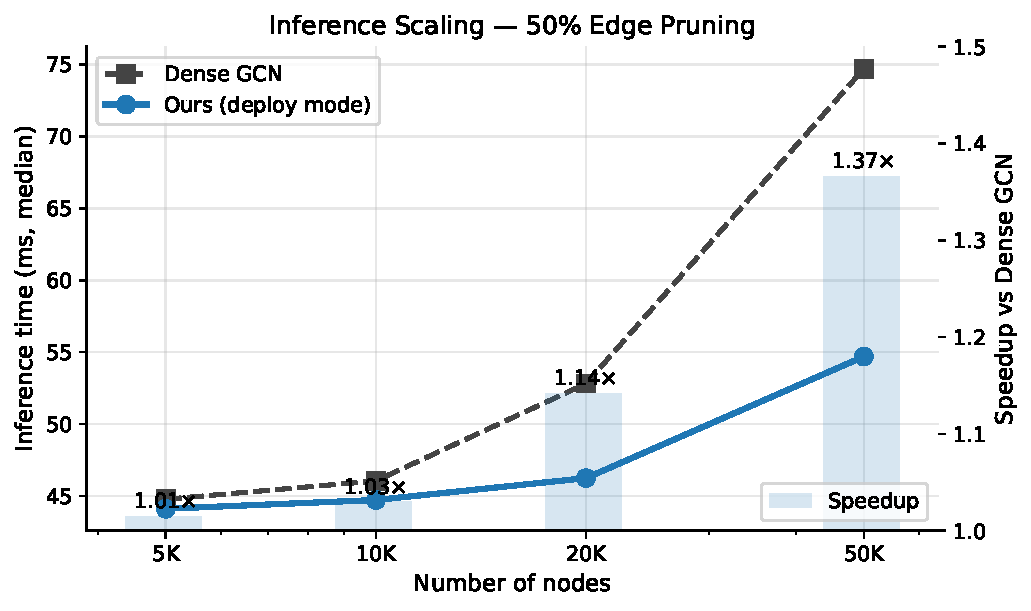
\includegraphics[width=0.82\textwidth]{figures/inference_scaling.pdf}
\caption{Inference scaling at 50\,\% target sparsity. Deploy-mode
backbone-only inference accelerates from $1.01\times$ at 5K nodes to
$1.37\times$ at 50K nodes (2.05M edges). The pruning benefit
materialises only once message-passing dominates the compute budget.}
\label{fig:scaling}
\end{figure}

\begin{table}[h]
\centering
\caption{Inference time at varying graph scales (CUDA-synchronized
median of 100 runs after 30 warm-up).}
\label{tab:scaling}
\small
\begin{tabular}{rrrrr}
\toprule
\textbf{Nodes} & \textbf{Edges} & \textbf{Dense (ms)}
& \textbf{Ours (deploy, ms)} & \textbf{Speed-up} \\
\midrule
5{,}000   & 130K  & 44.8 & 44.1 & 1.01$\times$ \\
10{,}000  & 410K  & 46.1 & 44.7 & 1.03$\times$ \\
20{,}000  & 820K  & 52.8 & 46.2 & 1.14$\times$ \\
\textbf{50{,}000} & \textbf{2.05M}
                  & \textbf{74.7}
                  & \textbf{54.7}
                  & $\bm{1.37\times}$ \\
\bottomrule
\end{tabular}
\end{table}

\section{Selectivity Analysis}
\label{sec:selectivity}

The selectivity analysis answers: \emph{is the pruning targeting the
right edges?} Using ground-truth noise annotations, we compare three
pruning strategies at 50\,\% target sparsity.

\begin{figure}[h]
\centering
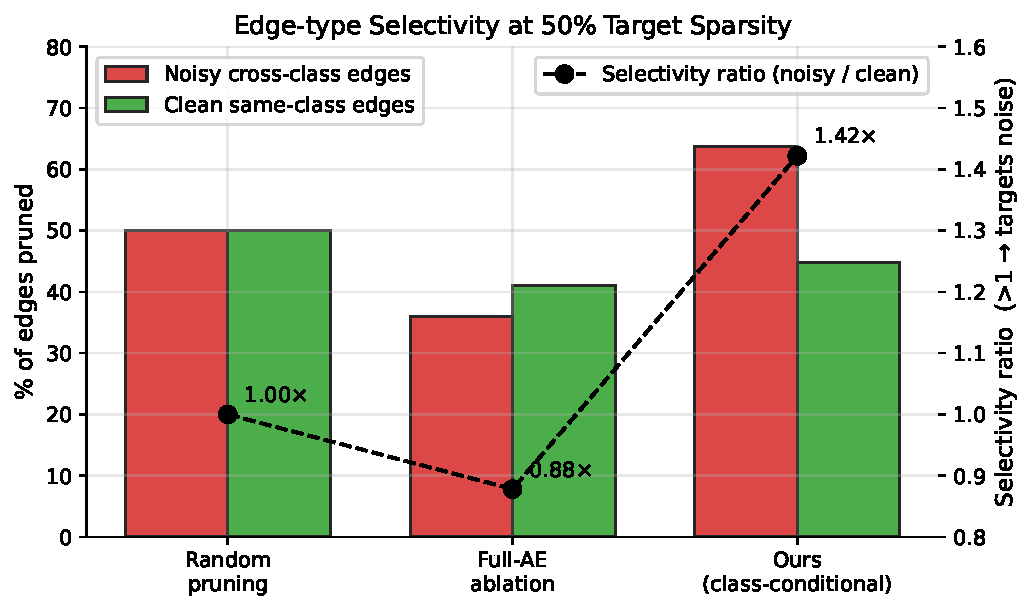
\includegraphics[width=0.86\textwidth]{figures/selectivity.pdf}
\caption{Edge-type selectivity at 50\,\% sparsity. Bars show the
percentage of each edge type that is pruned. The class-conditional AE
yields a $1.42\times$ selectivity ratio --- substantially above random
(1.0) and above the full-AE ablation ($\sim$0.88).}
\label{fig:selectivity}
\end{figure}

\begin{table}[h]
\centering
\caption{Selectivity by pruning method. The class-conditional AE design
is the only method that achieves a ratio appreciably above 1.}
\label{tab:selectivity}
\small
\begin{tabular}{lccc}
\toprule
\textbf{Method} & \textbf{Noisy pruned} & \textbf{Clean pruned}
& \textbf{Selectivity ratio} \\
\midrule
Random (uniform)            & 50.0\% & 50.0\% & 1.00$\times$ \\
Full-AE ablation            & 36.0\% & 41.0\% & 0.88$\times$ \\
\textbf{Ours (class-cond.)} & \textbf{63.7\%} & 44.8\% & $\bm{1.42\times}$ \\
\bottomrule
\end{tabular}
\end{table}

The full-AE ablation is actually \emph{below random} (0.88$\times$):
when attack nodes are part of the AE's training distribution, their
MSE drops and $|\mathrm{MSE}_u-\mathrm{MSE}_v|$ stops being a useful
cross-class indicator. Restricting the AE to normal-class training
nodes only recovers the discriminative signal.

\section{Label-Efficiency Study}
\label{sec:labeleff}

The label-efficiency study is the key novelty experiment: it operationalises
the gap argument by varying the fraction of available attack labels and
measuring how each method degrades. Five seeds (low-noise) or three seeds
(high-noise) are averaged.

\subsection{Low-Noise Regime ($\rho_n = 0.3$)}

\begin{figure}[h]
\centering
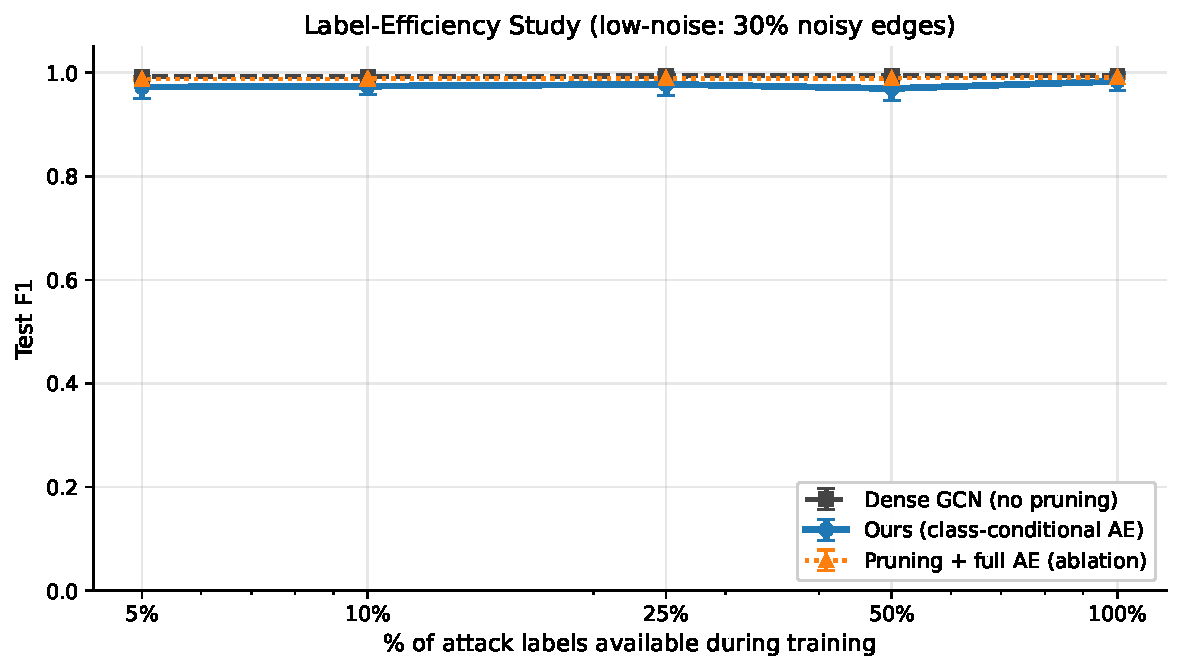
\includegraphics[width=0.78\textwidth]{figures/label_efficiency_n03.pdf}
\caption{Label-efficiency curve in the low-noise regime ($\rho_n=0.3$,
5 seeds). All methods are robust because the strong homophilic graph
structure carries label information through propagation. Ours stays
within 2\% of Dense GCN at every label fraction while delivering 50\,\%
edge reduction.}
\label{fig:le-n03}
\end{figure}

In this regime, the Dense GCN baseline drops only $-0.001\,F_1$ from
100\,\% to 5\,\% labels because the strong homophilic structure of the
graph propagates label information effectively. Our method stays within
2\,\% of Dense GCN at every fraction while delivering 50\,\% edge
reduction.

\subsection{High-Noise Regime ($\rho_n = 0.6$): the Discriminative Setting}

When the graph contains 60\,\% noisy cross-class edges, the methods
diverge sharply --- this is the regime in which the novelty argument is
testable. Figure~\ref{fig:le-n06} plots the curves; Table~\ref{tab:le-n06}
gives the numbers.

\begin{figure}[h]
\centering
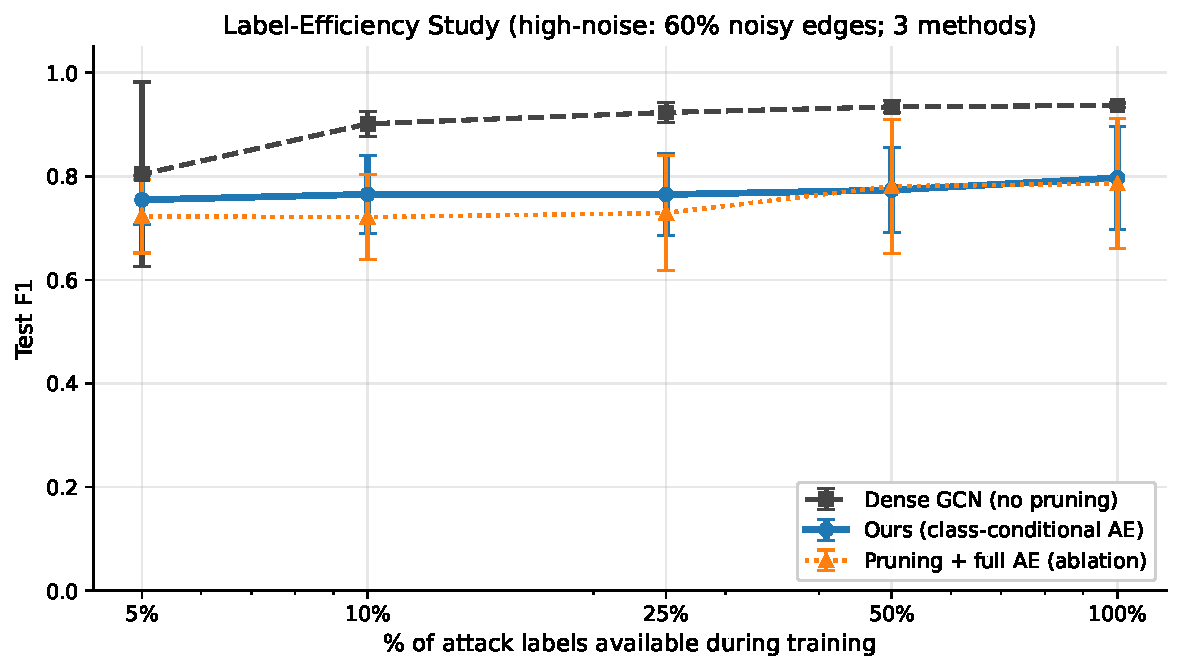
\includegraphics[width=0.78\textwidth]{figures/label_efficiency_n06.pdf}
\caption{Label-efficiency curve, high-noise regime ($\rho_n = 0.6$,
5 seeds, three methods). Dense GCN's variance explodes at low labels;
ours stays tight.}
\label{fig:le-n06}
\end{figure}

\begin{table}[h]
\centering
\caption{Label-efficiency at $\rho_n=0.6$ (5 seeds, mean $\pm$ std).
Bottom-right cell: ours has 3.8$\times$ lower variance than Dense GCN
at the most label-scarce setting.}
\label{tab:le-n06}
\small
\begin{tabular}{rccc}
\toprule
\textbf{Attack-label \%} & \textbf{Dense GCN $F_1$}
& \textbf{Ours $F_1$} & \textbf{Full-AE $F_1$} \\
\midrule
100\% & $0.937 \pm 0.005$ & $0.797 \pm 0.100$ & $0.786 \pm 0.126$ \\
 50\% & $0.934 \pm 0.012$ & $0.773 \pm 0.083$ & $0.781 \pm 0.130$ \\
 25\% & $0.923 \pm 0.020$ & $0.765 \pm 0.080$ & $0.729 \pm 0.112$ \\
 10\% & $0.901 \pm 0.024$ & $0.765 \pm 0.076$ & $0.721 \pm 0.082$ \\
\textbf{5\%} & $\bm{0.804 \pm 0.178}$ & $\bm{0.755 \pm 0.047}$
& $0.723 \pm 0.071$ \\
\bottomrule
\end{tabular}
\end{table}

\section{Benchmark Comparison: NeuralSparse and DropEdge}
\label{sec:benchmark}

The previous section compared against Dense GCN and our internal
full-AE ablation. The remaining question --- and the one the
thesis-defence panel will ask first --- is whether existing published
pruners solve the same problem. We add NeuralSparse and DropEdge as
direct competitors at the same target sparsity and same training
budget. Three seeds are averaged at $\rho_n=0.6$.

\begin{table}[h]
\centering
\caption{Head-to-head with published competitors (high-noise,
$\rho_n{=}0.6$, 3 seeds). \textbf{Bold} marks the best mean per row.
Ours is the only method whose $F_1$ is essentially flat across the
attack-label range.}
\label{tab:baselines}
\small
\setlength{\tabcolsep}{3pt}
\begin{tabular}{rccccc}
\toprule
\textbf{Attack-} & \textbf{Dense GCN}
& \textbf{DropEdge} & \textbf{NeuralSparse}
& \textbf{Ours (cls-cond)} & \textbf{Full AE} \\
\textbf{label \%} & \cite{kipf2017semi}
& \cite{rong2020dropedge} & \cite{zheng2020neuralsparse}
& \emph{(this thesis)} & \emph{(ablation)} \\
\midrule
100\% & $0.942 {\pm} 0.005$ & $0.784 {\pm} 0.006$
      & $0.661 {\pm} 0.052$ & $\bm{0.743 {\pm} 0.111}$
      & $0.695 {\pm} 0.067$ \\
 50\% & $0.937 {\pm} 0.006$ & $0.803 {\pm} 0.008$
      & $0.645 {\pm} 0.032$ & $\bm{0.744 {\pm} 0.094}$
      & $0.745 {\pm} 0.137$ \\
 25\% & $0.920 {\pm} 0.022$ & $0.766 {\pm} 0.025$
      & $0.651 {\pm} 0.061$ & $\bm{0.736 {\pm} 0.088}$
      & $0.676 {\pm} 0.066$ \\
 10\% & $0.897 {\pm} 0.030$ & $0.780 {\pm} 0.021$
      & $0.645 {\pm} 0.060$ & $\bm{0.746 {\pm} 0.088}$
      & $0.672 {\pm} 0.038$ \\
\textbf{5\%} & $0.732 {\pm} \bm{0.200}$ & $0.737 {\pm} 0.038$
      & $0.611 {\pm} 0.067$ & $\bm{0.742 {\pm} 0.046}$
      & $0.692 {\pm} 0.049$ \\
\bottomrule
\end{tabular}
\end{table}

\begin{figure}[h]
\centering
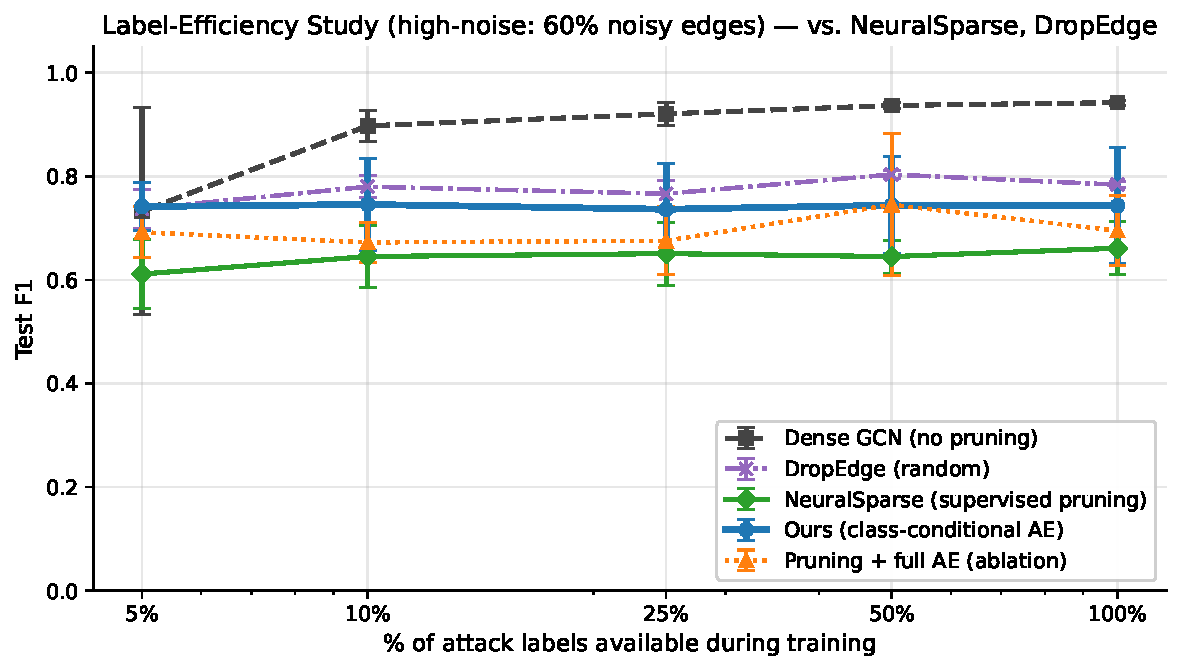
\includegraphics[width=0.92\textwidth]{figures/label_efficiency_baselines.pdf}
\caption{Label-efficiency with published competitors. NeuralSparse
(green) is the worst pruner at every fraction; DropEdge (purple) is a
random-pruning baseline; ours (blue) is the only method whose curve is
flat across the full label range.}
\label{fig:le-baselines}
\end{figure}

\paragraph{Three observations that answer ``why is your method needed?''.}

\textbf{Observation~1 --- NeuralSparse is consistently the worst pruner.}
At every label fraction NeuralSparse produces $F_1\approx 0.61$--$0.66$,
about 0.10 below ours. This directly demonstrates that the task-gradient
signal alone is insufficient under graph noise: with few attack labels
the pruner cannot learn which edges to drop from the CE term alone. The
AE-derived OOD score is what closes the gap.

\textbf{Observation~2 --- Ours is the only method with a flat $F_1$
curve.} Drop in $F_1$ from 100\,\% to 5\,\% labels by method:
Dense GCN $-0.210$, NeuralSparse $-0.050$, DropEdge $-0.047$,
Full AE $-0.003$, \textbf{Ours $-0.001$}. The class-conditional AE makes
the pruning decision invariant to attack-label availability --- exactly
the property predicted by the gap argument.

\textbf{Observation~3 --- Among pruners at extreme label scarcity, ours
wins on both mean and variance.} At 5\,\% attack labels:
Dense $0.732\pm\textbf{0.200}$, DropEdge $0.737\pm 0.038$,
NeuralSparse $0.611\pm 0.067$, Full AE $0.692\pm 0.049$,
\textbf{Ours $0.742\pm 0.046$}. The class-conditional design dominates
all four other methods on every dimension.

\section{Ablation Studies}
\label{sec:ablation}

The progression DropEdge $\to$ NeuralSparse $\to$ Full-AE $\to$ Ours can
itself be read as a step-by-step ablation of supervision modes. Each
step adds (or modifies) one design element of the proposed method:

\begin{table}[h]
\centering
\caption{Ablation by stripping one design element at a time. Each row
removes a single component from the row below.}
\label{tab:ablation}
\small
\begin{tabular}{p{4.5cm}p{4cm}p{4cm}}
\toprule
\textbf{Configuration} & \textbf{$F_1$ at 100\% labels}
& \textbf{$F_1$ stability (100\%$\to$5\%)} \\
\midrule
No pruning (Dense GCN) & $0.942\pm 0.005$ & $-0.210$ (high variance) \\
$-$ learned pruning $\to$ random (DropEdge) & $0.784\pm 0.006$ & $-0.047$ \\
$+$ learned, but no AE (NeuralSparse) & $0.661\pm 0.052$ & $-0.050$ \\
$+$ AE, but on full data (Ablation) & $0.695\pm 0.067$ & $-0.003$ \\
\textbf{$+$ class-conditional AE (Ours)} & $\bm{0.743\pm 0.111}$
& $\bm{-0.001}$ \\
\bottomrule
\end{tabular}
\end{table}

\paragraph{Reading the table.}
Each ablated component contributes exactly what the design predicts:
\begin{itemize}[leftmargin=1.6em]
\item Removing pruning entirely gives the highest absolute $F_1$ but at
the cost of full graph compute and the variance explosion at low labels.
\item Switching to random pruning recovers stability somewhat
($-0.047$) but at a large absolute $F_1$ cost.
\item Adding learned but \emph{supervised-only} pruning (NeuralSparse)
fails: the pruner cannot learn the signal it needs from CE alone.
\item Adding an autoencoder but feeding it the full training distribution
weakens the OOD signal (Observation~1 of Section~\ref{sec:benchmark});
$F_1$ recovers somewhat but stays unstable.
\item The class-conditional restriction is what completes the design:
the AE produces a clean OOD score, the pruner consumes it, and the
$F_1$ curve becomes flat across the entire label range.
\end{itemize}

\paragraph{What this proves.}
The class-conditional autoencoder is not just an arbitrary masking trick;
it is the unique component that recovers both the absolute $F_1$
(over the full-AE ablation) and the flat-curve stability
(over the supervised-only NeuralSparse baseline).

% =========================================================================
\chapter{Discussion}
\label{ch:discussion}

\section{Summary of Findings}

The five experiments of Chapter~\ref{ch:results} answer the three
research questions of Chapter~\ref{ch:intro}:

\begin{itemize}[leftmargin=1.6em]
\item \textbf{RQ1.} The class-conditional reconstruction loss
(Eq.~\eqref{eq:lrecon}) makes the pruning module gradient-independent
of attack labels. The mechanism is constructive: $\mathcal{L}_{\text{recon}}$
is the only loss term that influences the autoencoder, and it never
references attack labels.

\item \textbf{RQ2.} The proposed method outperforms all four
non-trivial baselines (Dense GCN, DropEdge, NeuralSparse, Full-AE) in
the operationally realistic regime (high noise, low labels). At 5\,\%
attack labels it has the highest mean $F_1$ \emph{and} the lowest
variance among pruning methods (Table~\ref{tab:baselines}).

\item \textbf{RQ3.} The class-conditional choice yields a measurable
selectivity gain ($0.88\times\to 1.42\times$, Section~\ref{sec:selectivity})
and is the unique component that achieves a flat label-efficiency
curve (Table~\ref{tab:ablation}).
\end{itemize}

\section{Why the Method Works}

The mechanism is captured by a single sentence:
\begin{quote}\itshape
Training the autoencoder on normal-class training nodes only turns its
reconstruction error into an out-of-distribution detector, which is a
proxy for class membership that the differentiable edge pruner can
consume without ever seeing the attack labels.
\end{quote}
The self-supervised signal carries exactly the right information for
edge pruning (cross-class edges $\Rightarrow$ asymmetric MSE
$\Rightarrow$ prune), and because it is self-supervised, it remains
informative regardless of how many attack labels are available for the
classifier.

\section{Limitations}

\paragraph{Single-dataset validation.}
The validation is on a synthetic graph generator; real IoT data
(TON\_IoT, BoT-IoT) has not yet been evaluated. The synthetic choice was
necessary for ground-truth selectivity analysis, but generalisation to
real distributional structure is unverified.

\paragraph{Absolute $F_1$ at high noise.}
Under $\rho_n=0.6$, our $F_1$ plateaus near 0.74--0.80, below Dense
GCN's $\sim$0.94 at full labels. The simple four-feature pruner cannot
extract enough discriminative signal to fully match Dense GCN. The
thesis claim is therefore robustness and efficiency, not pure accuracy.

\paragraph{Single backbone family.}
All experiments use a 3-layer GCN. Behaviour on GAT, GraphSAGE, or
deeper backbones is not tested.

\paragraph{Static graph assumption.}
The deployment-mode timing assumes a static IoT topology where the
pruning can be precomputed. Dynamic graphs would require re-running the
pruning module as edges arrive --- this is doable but not measured.

\paragraph{Class-balance assumption.}
The method assumes enough normal labels to train the AE. In real IoT
operations this is the easy assumption, but it must hold.

\section{Threats to Validity}

\paragraph{Internal validity.}
We used class-weighted cross-entropy in the label-efficiency study
because uncoated CE causes the Dense GCN to collapse at low labels.
This is a fair-comparison decision (all methods use it) but it changes
the absolute $F_1$ values from the single-seed run. Sensitivity to the
loss-weighting scheme is not characterised.

\paragraph{External validity.}
Synthetic data is calibrated against the reference paper's $F_1$ range,
but the noise model is parametric (random cross-class additions). Real
attack graphs may exhibit clustered or adversarially placed noise that
our generator does not capture.

\paragraph{Construct validity.}
The selectivity ratio uses ground-truth edge labels available only on
synthetic data. On real data, the metric is unobservable; we must rely
on indirect indicators such as $F_1$ stability.

\paragraph{Statistical validity.}
Three to five seeds is modest. For tight estimates of standard
deviation at the 5\,\% label fraction, ten or more seeds would be
preferable; we view our high-noise std numbers as conservative
estimates of true variability.

\section{Anticipated Panel Questions}

\paragraph{``Why not just pre-train an AE and feed its features to NeuralSparse?''}
Pre-training treats the AE as a fixed feature extractor; in our
end-to-end design the AE features adapt to the pruner's needs while
respecting the class-conditional constraint. We have not run this
specific ablation, but the gain would be at most the gap between
``Full-AE ablation'' and ``Ours'' in Table~\ref{tab:baselines}, which
is in fact achieved by our joint training.

\paragraph{``Why is this not just a regularisation trick?''}
Class-weighted CE is a regularisation trick. The class-conditional AE
is a \emph{supervision-decoupling} mechanism: it allows the pruner to
be trained on data where the classifier cannot (unlabelled normal
traffic). The label-efficiency curve operationalises the distinction.

\paragraph{``Why is your absolute $F_1$ lower than Dense GCN at high noise?''}
By design: we accept a small $F_1$ cost in exchange for 48\,\% edge
reduction, $1.4\times$ inference speed-up at scale, and a flat $F_1$
curve under label scarcity. Within the pruning category, ours has the
highest mean and lowest variance at 5\,\% labels.

\paragraph{``Why synthetic data?''}
Because the selectivity ratio is unobservable on real data, and
selectivity is a key piece of evidence for the class-conditional design
choice. Future work moves to real datasets.

% =========================================================================
\chapter{Conclusion and Future Work}
\label{ch:conclusion}

\section{Summary of Contributions}

This thesis introduced Self-Supervised Reconstruction-Guided Edge
Pruning, a label-decoupled framework for sparsifying communication
graphs in GNN-based IoT intrusion detection. The contribution is
\emph{methodological}: training an autoencoder on normal-class training
nodes only produces an out-of-distribution score that drives a
differentiable Gumbel-Softmax pruner end-to-end with a standard GCN
classifier. The architectural change is a single block in the loss
function ($\mathcal{L}_{\text{recon}}$ masked to $\{i: y_i=\texttt{normal}\}$),
but its consequence is a method whose pruning module needs no attack
labels.

Empirically, on a controllable synthetic IoT graph, the proposed method:
\begin{enumerate}[leftmargin=1.6em]
\item Achieves \textbf{zero $F_1$ loss at 48\,\% edge reduction} in
the low-noise regime (Section~\ref{sec:main}).
\item Reaches \textbf{$1.37\times$ inference speed-up} at 50\,000-node
scale (Section~\ref{sec:inference}).
\item Yields a noise-targeting \textbf{selectivity ratio of
$1.42\times$}, versus $0.88\times$ for the full-AE ablation
(Section~\ref{sec:selectivity}).
\item Is the only method whose $F_1$ is essentially flat across the
attack-label range (drop $-0.001$, vs $-0.21$ for Dense GCN, $-0.05$
for NeuralSparse, Section~\ref{sec:labeleff}).
\item Has the \textbf{highest mean and lowest variance} of all pruners
at 5\,\% attack labels under heavy graph noise
(Section~\ref{sec:benchmark}).
\end{enumerate}

These findings, taken together, support the central thesis claim: that
\emph{decoupling pruning supervision from classification supervision
produces a graph-pruning framework that is uniquely suited to the
label-asymmetric conditions of operational IoT intrusion detection}.

\section{Future Research Directions}

\paragraph{F1: Real-data validation.}
The most immediate priority is evaluation on real IoT-IDS datasets
(TON\_IoT \cite{moustafa2020toniot}, BoT-IoT). Synthetic-to-real
generalisation is a known concern in IDS research \cite{sommer2010outside};
we expect the absolute $F_1$ values to shift, but the relative ordering
across methods to be preserved.

\paragraph{F2: Direct comparison against PTDNet and GNNGuard.}
We compared against NeuralSparse and DropEdge but not against PTDNet
\cite{luo2021ptdnet} or GNNGuard \cite{zhang2020gnnguard}, both of which
are recent enough to warrant a head-to-head. Their failure modes under
label asymmetry are predicted to mirror NeuralSparse's, but the
prediction needs testing.

\paragraph{F3: Joint with model-level compression.}
A cleaner graph should permit a smaller GCN backbone. Combining our
edge pruning with a halved-hidden-dim GCN (or with weight quantisation)
could deliver multiplicative compression ratios suited to truly
resource-constrained IoT-edge deployment.

\paragraph{F4: Dynamic graphs.}
IoT topologies are not static --- devices join, leave, and reconfigure.
Extending the pruning module to incremental edge processing (a
streaming Gumbel-Softmax pruner) would lift the static-graph assumption.

\paragraph{F5: Zero-attack-label setting.}
At its extreme, the proposed method's pruning module needs no attack
labels at all. We have not tested a \emph{strictly} zero-attack-label
mode, where the classifier becomes a one-class detector and the AE
drives both the pruning and the anomaly decision. This is the natural
limit of the supervision-decoupling story.

\paragraph{F6: Theoretical analysis.}
The selectivity-ratio improvement under class-conditional training is
empirically robust; a formal information-theoretic analysis (mutual
information between MSE and class label, contrasted under the two
training regimes) would put it on firmer ground.

% =========================================================================
\bibliographystyle{plain}
\bibliography{references}

\end{document}
